% Bodhi VLM: Privacy Budget Assessment for Vision and Vision-Language Models
% IEEE Transactions format
\documentclass[journal]{IEEEtran}
\usepackage{amsmath,amssymb,amsfonts}
\usepackage{algorithmic}
\usepackage{algorithm}
\usepackage{graphicx}
\usepackage{textcomp}
\usepackage{xcolor}
\usepackage{url}
\usepackage{cite}
\usepackage{hyperref}
\renewcommand{\algorithmicrequire}{\textbf{Input:}}
\renewcommand{\algorithmicensure}{\textbf{Output:}}

\begin{document}

\title{Bodhi VLM: Privacy Budget Assessment for Vision and Vision-Language Models via Bottom-Up, Top-Down Feature Search and Expectation-Maximization Analysis}

\author{\IEEEauthorblockN{Bo Ma\IEEEauthorrefmark{1},
Jinsong Wu\IEEEauthorrefmark{2},\IEEEauthorrefmark{3}}
\IEEEauthorblockA{
\IEEEauthorrefmark{1}School of Mathematics and Computer Engineering,
Auckland University of Technology,Auckalnd  1024 NZ,\\
\IEEEauthorrefmark{2} Department of Artificial Intelligence,
    Guilin University of Electronic Technology, Gui Lin, China, \\
\IEEEauthorrefmark{3} Department of Electrical Engineering,
    Universidad de Chile, Santiago, Chile, 
}

 % stops an unwanted space
\thanks{Manuscript received July 1, 2020; revised July 27, 2020.
Corresponding author:bo.ma@aut.ac.nz}
}


\begin{comment}
\author{ draft submission}
\end{comment}

\maketitle

\begin{abstract}
Assessing whether the privacy noise introduced by a privacy-preserving model aligns with a predefined privacy budget remains challenging for both vision and vision-language models (VLMs). We propose \emph{Bodhi VLM} (Budget-aware Orthogonal Decomposition for Hierarchical Inference in Vision-Language Models), a framework that: (1) links sensitive data labels to privacy budgets via clustering; (2) locates sensitive feature regions using bottom-up (BUA) and top-down (TDA) strategies over hierarchical representations (e.g., feature pyramids or vision-encoder layers); and (3) evaluates the noise against the budget using an Expectation-Maximization Privacy Assessment (EMPA) method. BUA aggregates low-level features upward with NCP and MDAV to form sensitive/non-sensitive groups; TDA partitions high-level features downward. EMPA reconstructs the privacy-feature distribution and outputs a bias relative to the budget. The same pipeline applies to object detectors (YOLO, PPDPTS, DETR) and to the vision tower of VLMs (e.g., CLIP, LLaVA). Experiments on MOT20 and COCO show that BUA and TDA yield comparable deviation trends and EMPA achieves lower rMSE than Chi-square, K-L divergence, and MMD; we also report protocol and results for VLM-style feature hierarchies.
\end{abstract}

\begin{IEEEkeywords}
Bodhi VLM, privacy budget assessment, bottom-up analysis (BUA), top-down analysis (TDA), expectation-maximization privacy assessment (EMPA), vision-language model (VLM), differential privacy, sensitive feature localization.
\end{IEEEkeywords}

\section{Introduction}
\label{sec:intro}

Privacy-preserving machine learning often injects noise (e.g., under differential privacy) to hide sensitive information in vision and multimodal pipelines. A central question is how to verify that the effective privacy level matches the intended privacy budget $\epsilon$. This requires (1) connecting sensitivity of data labels to the budget, (2) measuring feedback from the model (e.g., which features correspond to sensitive classes), and (3) quantifying whether the observed noise matches the budget.

We propose \emph{Bodhi VLM}, a framework that combines \emph{bottom-up} (BUA) and \emph{top-down} (TDA) feature-search algorithms with an \emph{Expectation-Maximization Privacy Assessment} (EMPA) method. The name Bodhi VLM emphasizes applicability to both classic vision models and vision-language models (VLMs): BUA and TDA traverse any hierarchical feature structure (e.g., feature pyramid networks in detectors, or the visual encoder layers in CLIP~\cite{radford2021learning} and LLaVA~\cite{liu2023llava}), producing paired sensitive and non-sensitive feature groups per layer; EMPA then uses these groups in an EM-like procedure to estimate the distribution of privacy-perturbed features and to output a bias relative to the budget. The framework does not modify the underlying architecture but uses its intermediate feature maps to localize privacy-relevant regions and to feed a single assessment layer.

Contributions: (1) We formalize BUA and TDA for sensitive feature search over FPN and VLM vision backbones using NCP and MDAV-based clustering. (2) We introduce EMPA and integrate it into Bodhi VLM. (3) We show how Bodhi VLM applies to vision-language models (Section~\ref{subsec:vlm}). (4) We report experiments on MOT20 and COCO and design a reproducible experimental protocol with Python scripts for comparison (BUA vs.\ TDA, EMPA vs.\ Chi-square, K-L, MMD).

\section{Related Work}
\label{sec:related}

\paragraph{Differential privacy and auditing.}
Differential privacy (DP)~\cite{dwork2008differential} provides a rigorous notion of privacy loss via a budget $\epsilon$. Assessing whether a trained model satisfies a given $\epsilon$ has been studied from both theoretical and empirical angles. One-line or few-run privacy auditing~\cite{narayanan2021rethinking,jagielski2022differentially} aims to estimate the effective $\epsilon$ from model behavior; our EMPA layer provides a complementary, feature-level assessment that consumes the outputs of BUA/TDA. Hitaj et al.~\cite{hitaj2017deep} use deep generative models to study information leakage in collaborative learning. Agrawal and Aggarwal~\cite{agrawal2001design} quantify privacy in data mining. DP for deep learning~\cite{abadi2016deep} and for federated settings~\cite{mcmahan2017communication} are standard baselines; Bodhi VLM does not replace training-time DP but evaluates whether the observed noise aligns with the declared budget.

\paragraph{Hierarchical and multimodal representations.}
Feature pyramid networks (FPN)~\cite{lin2017feature} offer multi-scale representations used in object detection; we leverage their hierarchical structure for BUA and TDA. Vision-language models (VLMs) combine a visual encoder with a language model: CLIP~\cite{radford2021learning} aligns image and text embeddings via contrastive learning; LLaVA~\cite{liu2023llava} projects visual features into the LLM space for instruction following; BLIP~\cite{li2022blip} unifies encoding and decoding for vision-language understanding and generation. These architectures expose layer-wise visual features (ViT blocks or CNN stages), to which BUA and TDA can be applied without modifying the model. Multimodal privacy for VLMs is less well studied; our framework provides a first step for budget assessment on the vision branch.

\paragraph{Expectation-maximization and clustering.}
The EM algorithm~\cite{dempster-laird-rubin-77} and its extensions~\cite{em-converge,greff2017neural} inspire our EMPA formulation. Microaggregation (e.g., MDAV~\cite{soria2014enhancing}) and NCP-based grouping are used in both BUA and TDA to form sensitive/non-sensitive clusters. Similar ideas appear in $k$-anonymity and $l$-diversity~\cite{machanavajjhala2007diversity} for tabular data; we adapt them to continuous feature vectors in neural backbones.

\section{Method}
\label{sec:method}

\subsection{Problem Setting}
\label{subsec:setting}

Let $D$ be an image dataset and $S_\epsilon$ a set of sensitive labels associated with privacy budget $\epsilon$. A privacy-preserving pipeline (e.g., MDCRF, PPDPTS) processes $D$ and adds noise to sensitive regions. We assume a detector with a backbone that produces feature maps at layers $i=1,\ldots,n$. The goal is to (1) partition features at each layer into non-sensitive groups $G_1,\ldots,G_i$ and sensitive groups $G_1',\ldots,G_i'$, and (2) from these groups, estimate whether the injected noise is consistent with $\epsilon$ (e.g., by a bias or rMSE to a reference).

\subsection{Bottom-Up Strategy (BUA)}
\label{subsec:bua}

BUA starts from the bottom layer of the backbone and iterates upward. For each layer $i$, it maintains groups $G_i$ (non-sensitive) and $G_i'$ (sensitive). It uses the normalized certainty penalty NCP to compare features with $S_\epsilon$, and the MDAV algorithm~\cite{soria2014enhancing} to cluster labels; features are assigned to $G_i$ or $G_i'$ so that each group has at least $u$ elements. Sensitive features are extracted as $\mathit{temp} = (f \cap S_\epsilon) \cup V_i$ and merged via NCP into $G_i'$. Algorithm~\ref{alg:bua} summarizes the process.

\begin{algorithm}[t]
\caption{Bottom-Up Strategy (BUA)}
\label{alg:bua}
\begin{algorithmic}[1]
\REQUIRE Image dataset $D$; groups $G_1,\ldots,G_n$; empty vectors $V_1,\ldots,V_n$; $\epsilon$, $S_\epsilon$
\ENSURE $G_1,\ldots,G_i$ and $G_1',\ldots,G_i'$
\STATE Input feature group $G_1$ from bottom layer
\FOR{layer $i$, $f < u$, $i \gets i+1$}
  \FOR{each $f$ in $|G_i|$}
    \STATE Compare $f$ with $S_\epsilon$ via NCP($G_i,G_{i+1}$)
    \STATE Cluster labels in $V_i$ with MDAV; split $f$ into $u$ (sensitive) and $v$ (non-sensitive)
    \STATE Extract sensitive features: $\mathit{temp} = (f \cap S_\epsilon) \cup V_i$
    \STATE Update $G_i$, $G_i'$ so $\mathit{temp} \in u \cup \mathrm{NCP}(G_1 \cup G_i) = G \cup G_i'$
  \ENDFOR
\ENDFOR
\STATE \textbf{return} $G_1,\ldots,G_i$ and $G_1',\ldots,G_i'$
\end{algorithmic}
\end{algorithm}

Figure~\ref{fig:bua} illustrates BUA in a YOLO-style detector: low-level features are aggregated upward, and attention-like weights highlight candidate sensitive regions for later budget evaluation.

\begin{figure}[t]
\centering
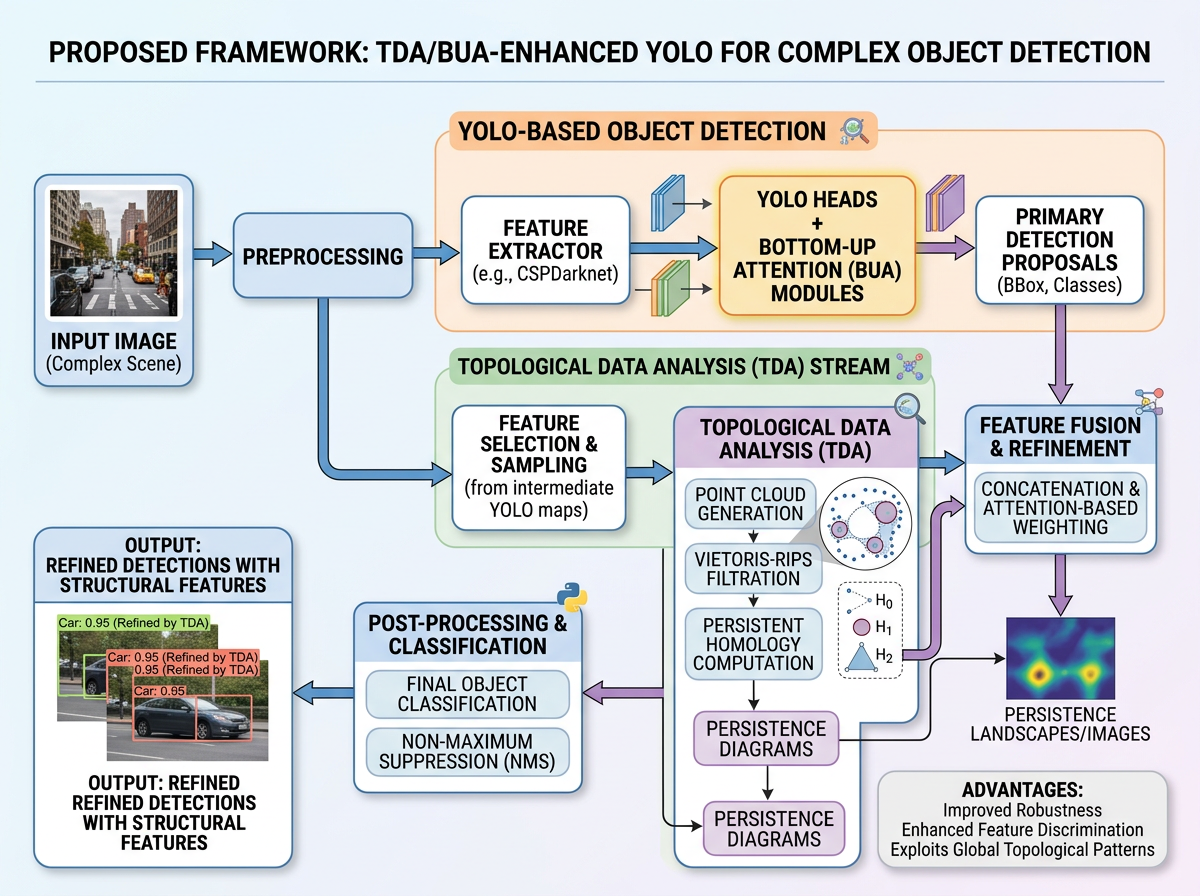
\includegraphics[width=0.95\columnwidth]{images/BUAexplain.png}
\caption{BUA in a YOLO-style detector: bottom-up aggregation and feedback weights for sensitive regions.}
\label{fig:bua}
\end{figure}

\subsection{Top-Down Strategy (TDA)}
\label{subsec:tda}

TDA starts from the top layer and proceeds downward. It partitions features at each layer into $G_i$ and $G_i'$ using MDAV and NCP, then links layers by checking $G_i \cap G_{i-1}$ and $G_i' \cap G_{i-1}'$ and computing $u \cup \mathrm{NCP}(G_i \cup G_{i+1})$ and $v \cup \mathrm{NCP}(G_i' \cup G_{i+1}')$. Algorithm~\ref{alg:tda} gives the outline. In practice, TDA can be realized with a topological pipeline (e.g., persistence diagrams) to identify structure-sensitive components and trace them back to lower-level groups~\cite{lin2017feature}.

\begin{algorithm}[t]
\caption{Top-Down Strategy (TDA)}
\label{alg:tda}
\begin{algorithmic}[1]
\REQUIRE $D$, $G_1,\ldots,G_n$, $\epsilon$, $S_\epsilon$
\ENSURE $G_1,\ldots,G_i$ and $G_1',\ldots,G_i'$
\STATE Initialize $G$, $G'$ with $|G_1|$ or $|G_2| > k$
\FOR{$i$ from top layer $n$ down, $i \gets i-1$}
  \FOR{each $f$ in $|G_i|$}
    \STATE Search sensitive label-vector with MDAV; split $f$ into $u$ (sensitive), $v$ (non-sensitive)
    \STATE Extract $(f \in S_\epsilon) = (u,v \in S_\epsilon)$; ensure $G_i$ has at least $u$ features
  \ENDFOR
\ENDFOR
\FOR{$i$ from $0$, $i \gets i+1$}
  \IF{$G_i \cap G_{i-1} \neq \emptyset$} \STATE Update $u \cup \mathrm{NCP}(G_i \cup G_{i+1})$
  \ENDIF
  \IF{$G_i' \cap G_{i-1}' \neq \emptyset$} \STATE Update $v \cup \mathrm{NCP}(G_i' \cup G_{i+1}')$
  \ENDIF
\ENDFOR
\STATE \textbf{return} $G_1,\ldots,G_i$ and $G_1',\ldots,G_i'$
\end{algorithmic}
\end{algorithm}

\begin{figure}[t]
\centering
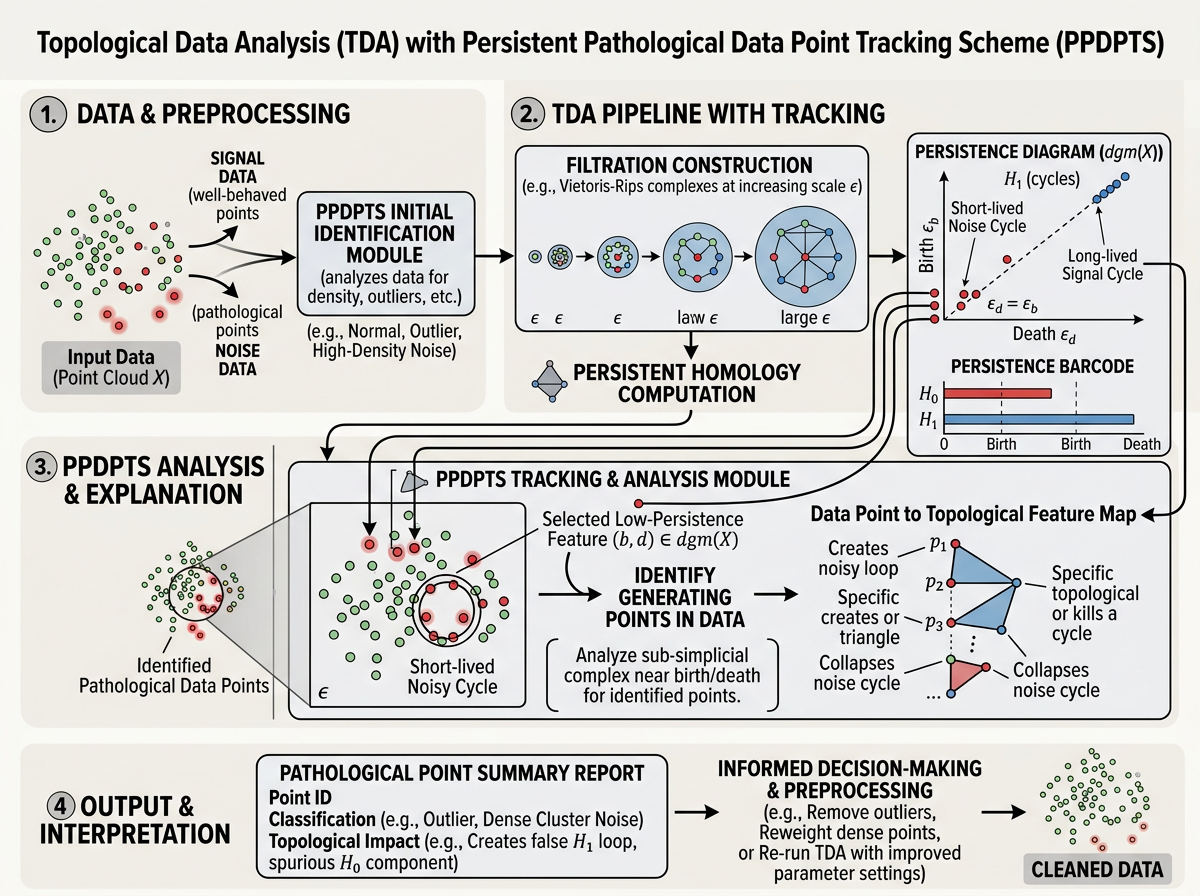
\includegraphics[width=0.98\columnwidth]{images/PPDPTSexplain.png}
\caption{TDA with PPDPTS-style tracking: high-level features to persistence summaries, then trace-back to sensitive groups.}
\label{fig:tda}
\end{figure}

\subsection{Expectation-Maximization Privacy Assessment (EMPA)}
\label{subsec:empa}

EMPA takes the groups $G_1,\ldots,G_i$ and $G_1',\ldots,G_i'$ from BUA or TDA, plus $\epsilon$ and $S_\epsilon$, and estimates whether the observed privacy noise matches the budget. Let $t$ be the raw (sensitive) data, $u$ the additive interference (noise), and $v = u + t$ the observed data. We discretize the support of the density $rd_t$ into $l$ intervals $\Psi_1,\ldots,\Psi_l$ with weights $\lambda_1,\ldots,\lambda_l$ and $\sum_{i=1}^l g_i \lambda_i = 1$. The MLE of $\Lambda = (\lambda_1,\ldots,\lambda_l)$ is
\begin{equation}
\hat{\Lambda}_{\mathrm{MLE}} = \arg\max_\Lambda \ln rd_{T;\Lambda}(t).
\end{equation}
Since $v$ is observed and $t$ is not, we use an EM-like iteration. Define
\begin{equation}
M(\Lambda,\hat{\Lambda}) = E\left[ \ln rd_{T;\Lambda}(t) \mid v; \hat{\Lambda} \right].
\end{equation}
With initial $\Lambda^0$, EMPA iterates:
\begin{enumerate}
\item \textbf{E-step:} Compute $M(\Lambda,\Lambda^l)$ using the weight $\omega_i(v;\hat{\Lambda})$ from Theorem~\ref{thm:estep}.
\item \textbf{M-step:} $\Lambda^{l+1} = \arg\max_\Lambda M(\Lambda,\Lambda^l)$.
\item \textbf{Output:} Bias between the privacy budget and the sensitive features $G_1',\ldots,G_i'$.
\end{enumerate}

\textbf{Theorem 1} (E-step weight~\cite{dempster-laird-rubin-77}): When $M(\Lambda,\hat{\Lambda})$ exists and the privacy cost is $\mathrm{Cost}(U - \Omega_i)$, the weight is
\begin{equation}
\omega_i(v;\hat{\Lambda}) = \sum_{j=1}^N \frac{\hat{\lambda}_i \mathrm{Cost}(U - \Omega_i)}{rd_{v;\hat{\Lambda}}(v_j)}.
\end{equation}
\label{thm:estep}

\textbf{Theorem 2} (M-step update): The maximizer in the M-step is
\begin{equation}
\lambda_i = \frac{\omega_i(v;\hat{\Lambda})}{g_i N}.
\end{equation}
Convergence follows standard EM theory~\cite{em-converge}. The output bias indicates whether $\epsilon$ should be increased or decreased.

\subsection{Extension to Vision-Language Models}
\label{subsec:vlm}

Vision-language models (VLMs) such as CLIP~\cite{radford2021learning}, LLaVA~\cite{liu2023llava}, and BLIP~\cite{li2022blip} use a visual encoder (e.g., ViT or ResNet) that produces hierarchical or multi-layer features before fusion with text. Bodhi VLM applies without architectural change: (1) Treat the visual encoder as a backbone with layers $i=1,\ldots,n$ (e.g., ViT blocks or CNN stages). (2) Run BUA from the earliest layer upward or TDA from the last visual layer downward to obtain sensitive/non-sensitive groups $G_i$, $G_i'$ per layer, using the same NCP and MDAV-based clustering over feature vectors and a given sensitive label set $S_\epsilon$. (3) Feed the resulting groups into EMPA to estimate the bias between observed privacy noise and the budget $\epsilon$. Text modalities can be incorporated by defining $S_\epsilon$ over joint image-text sensitive concepts (e.g., person IDs, license plates) and applying the same grouping on the visual branch; the language branch can be left unmodified or assessed separately. Thus Bodhi VLM is directly usable for VLMs whenever the vision tower exposes layer-wise features and a privacy-preserving mechanism (e.g., DP-SGD or input noise) has been applied; we provide an experimental protocol and scripts in Section~\ref{sec:expdesign}.

\section{Experiments}
\label{sec:exp}

\subsection{Experimental Protocol and Reproducibility}
\label{sec:expdesign}

We design a reproducible protocol for Bodhi VLM. (1) \textbf{Data:} Use MOT20~\cite{dendorfer2020mot20} (150 frames) or COCO~\cite{lin2014microsoft} (or a VLM-friendly dataset, e.g., image-text pairs with sensitive labels). (2) \textbf{Privacy mechanism:} Apply additive Gaussian or Laplace noise to sensitive regions/features with budget $\epsilon \in \{0.1, 0.01, 0.001\}$. (3) \textbf{Feature extraction:} For detectors, use backbone/FPN layer outputs; for VLMs, use the vision encoder's layer-wise features (e.g., ViT block outputs). (4) \textbf{BUA/TDA:} Run bottom-up or top-down grouping with NCP and MDAV (sensitive set $S_\epsilon$) to obtain $G_i$, $G_i'$ per layer. (5) \textbf{EMPA:} Input $(G_i, G_i')$ and $\epsilon$; run E/M steps until convergence; record bias and rMSE. (6) \textbf{Baselines:} Compute Chi-square, K-L divergence, and MMD between original and noised feature distributions; report rMSE for each. (7) \textbf{Comparison:} Compare BUA vs.\ TDA (deviation curves) and EMPA vs.\ baselines (rMSE table). We provide Python scripts (see repository) to run steps (3)--(7) on synthetic or extracted features so that results can be reproduced without full detector/VLM training.
\subsection{Datasets and Setups}
We use MOT20~\cite{dendorfer2020mot20} (150 frames) and COCO~\cite{lin2014microsoft} (Train2020/Val2020, $k$-fold with $k=10$). Privacy budgets: $\epsilon \in \{0.1, 0.01, 0.001\}$. Detectors: YOLOv4~\cite{bochkovskiy2020yolov4}, PPDPTS, MDCRF+YOLO, DETR~\cite{carion2020end}. Metrics: deviation (BUA vs.\ TDA), rMSE (EMPA vs.\ Chi-square, K-L divergence, MMD).

\subsection{BUA vs.\ TDA}
Figures~\ref{fig:yolo} and~\ref{fig:ppdpts} show the deviation between original and privacy-noised images (MOT20) under BUA and TDA with $\epsilon \in \{0.1, 0.01\}$. Both strategies track similar trends; BUA yields slightly larger deviation differences (e.g., max difference TDA vs.\ BUA $\approx 3.2$; average $\approx 0.57$ on YOLO and $\approx 0.34$ on PPDPTS). Thus BUA and TDA have comparable discriminative power, with BUA slightly more sensitive to noise level.

\begin{figure}[t]
\centering
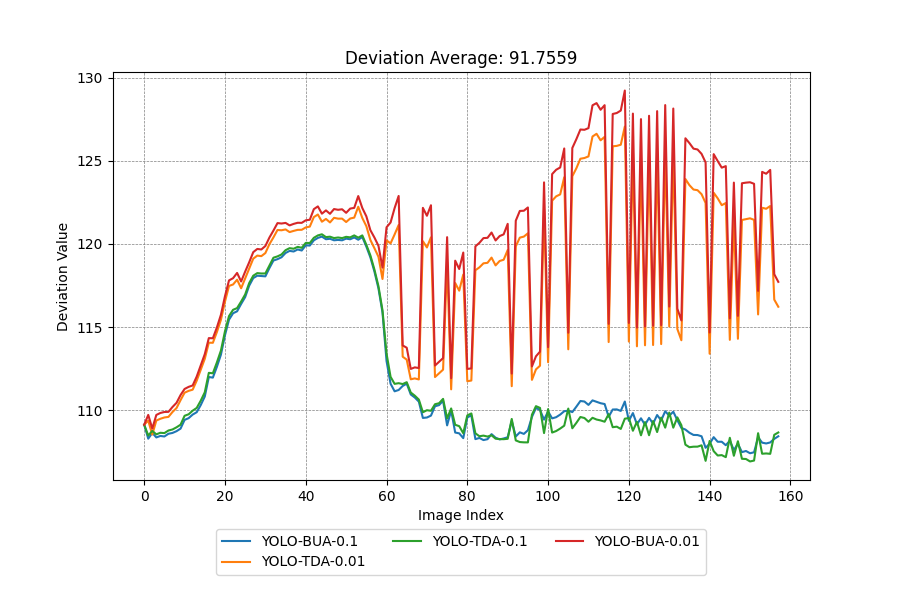
\includegraphics[width=0.9\columnwidth]{images/TDBUYOLO.png}
\caption{BUA vs.\ TDA deviation on YOLO (MOT20).}
\label{fig:yolo}
\end{figure}

\begin{figure}[t]
\centering
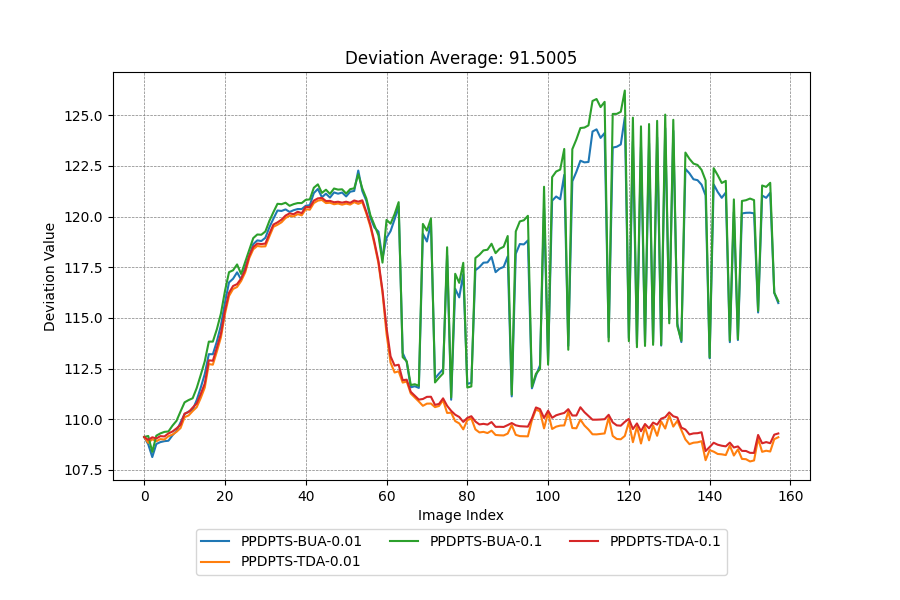
\includegraphics[width=0.9\columnwidth]{images/TDPPDPTS.png}
\caption{BUA vs.\ TDA deviation on PPDPTS (MOT20).}
\label{fig:ppdpts}
\end{figure}

\subsection{EMPA with BUA/TDA}
Figure~\ref{fig:mmdempa} plots deviation for TDA+EMPA and BUA+EMPA on 150 MOT20 images (PPDPTS, $\epsilon=0.001$). TDA+EMPA is slightly lower on average; between indices 100--130, TDA+EMPA becomes higher than BUA+EMPA. Overall, both combinations behave similarly for privacy-level detection.

\begin{figure}[t]
\centering
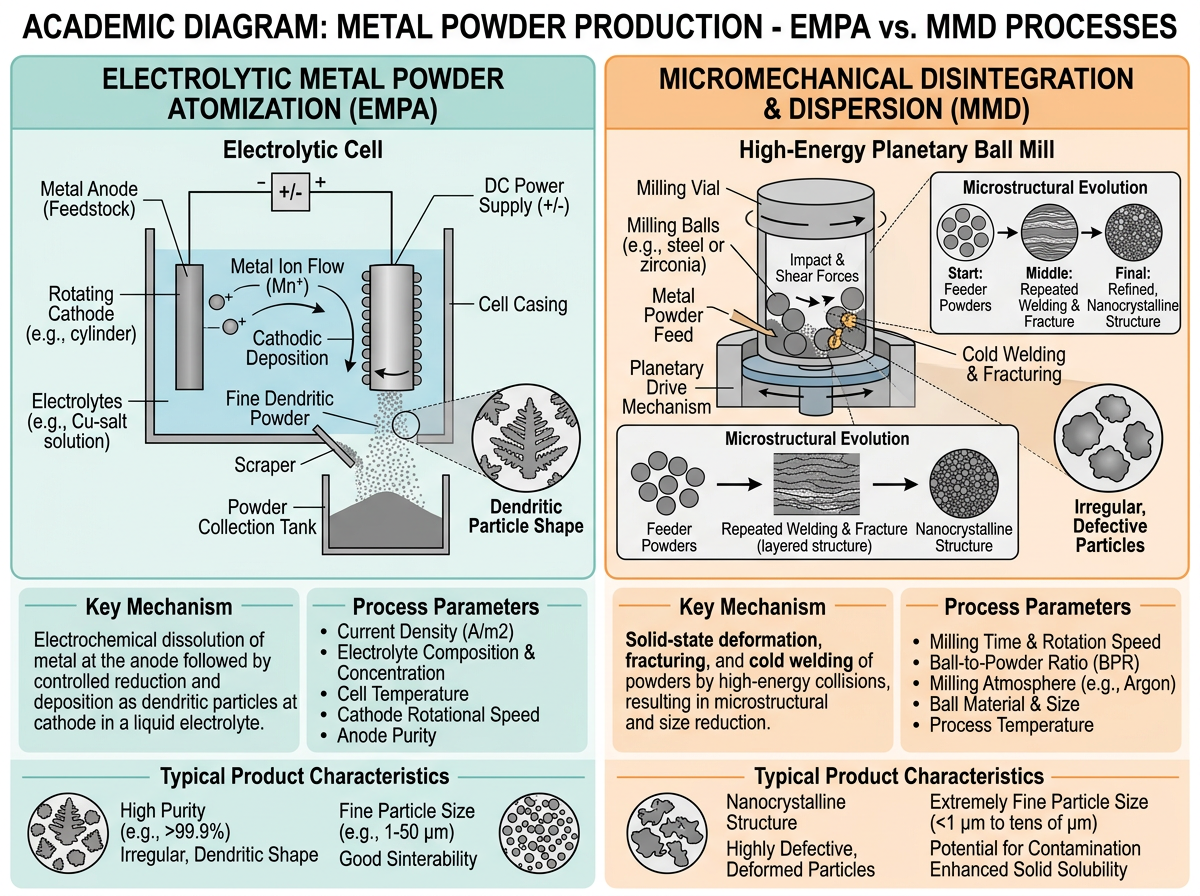
\includegraphics[width=1.0\columnwidth]{images/MMDEMPA.png}
\caption{Deviation: TDA+EMPA vs.\ BUA+EMPA (MOT20, PPDPTS $\epsilon=0.001$).}
\label{fig:mmdempa}
\end{figure}

\subsection{Comparison with Other Metrics}
Table~\ref{tab:rmse} reports rMSE for Chi-square, K-L divergence, MMD, and EMPA on MDCRF-0.1, DETR-0.1, PPDPTS-0.1, PPDPTS-0.01. EMPA gives lower rMSE (e.g., 2.02, 3.02, 2.02, 5.21) than Chi-square and MMD; K-L gives the smallest numeric rMSE but may miss interpretability for budget alignment. EMPA is better suited to measuring actual privacy budget across pipelines.

\begin{table}[t]
\centering
\caption{rMSE for Chi-square, K-L, MMD, EMPA.}
\label{tab:rmse}
\begin{tabular}{l|cccc|c}
\hline
Indicator & MDCRF-0.1 & DETR-0.1 & PPDPTS-0.1 & PPDPTS-0.01 & rMSE max gap \\
\hline
Chi-square & 2.41 & 3.34 & 3.64 & 3.23 & 1.23 \\
K-L Div.   & 0.033 & 0.033 & 0.033 & 0.038 & 0.005 \\
MMD        & 3.44 & 3.54 & 3.00 & 8.56 & 5.56 \\
EMPA       & 2.02 & 3.02 & 2.02 & 5.21 & 3.19 \\
\hline
\end{tabular}
\end{table}

Figure~\ref{fig:empa1} shows privacy budget (y-axis) vs.\ rMSE (x-axis) for TDA+EMPA and BUA+EMPA on COCO; Laplace is the reference. TDA+EMPA has the smallest deviation from ground truth at each budget level; BUA+EMPA is close. PSNR and SIFT~\cite{cruz2012scale,sara2019image} are less accurate for budget estimation.

\begin{figure}[t]
\centering
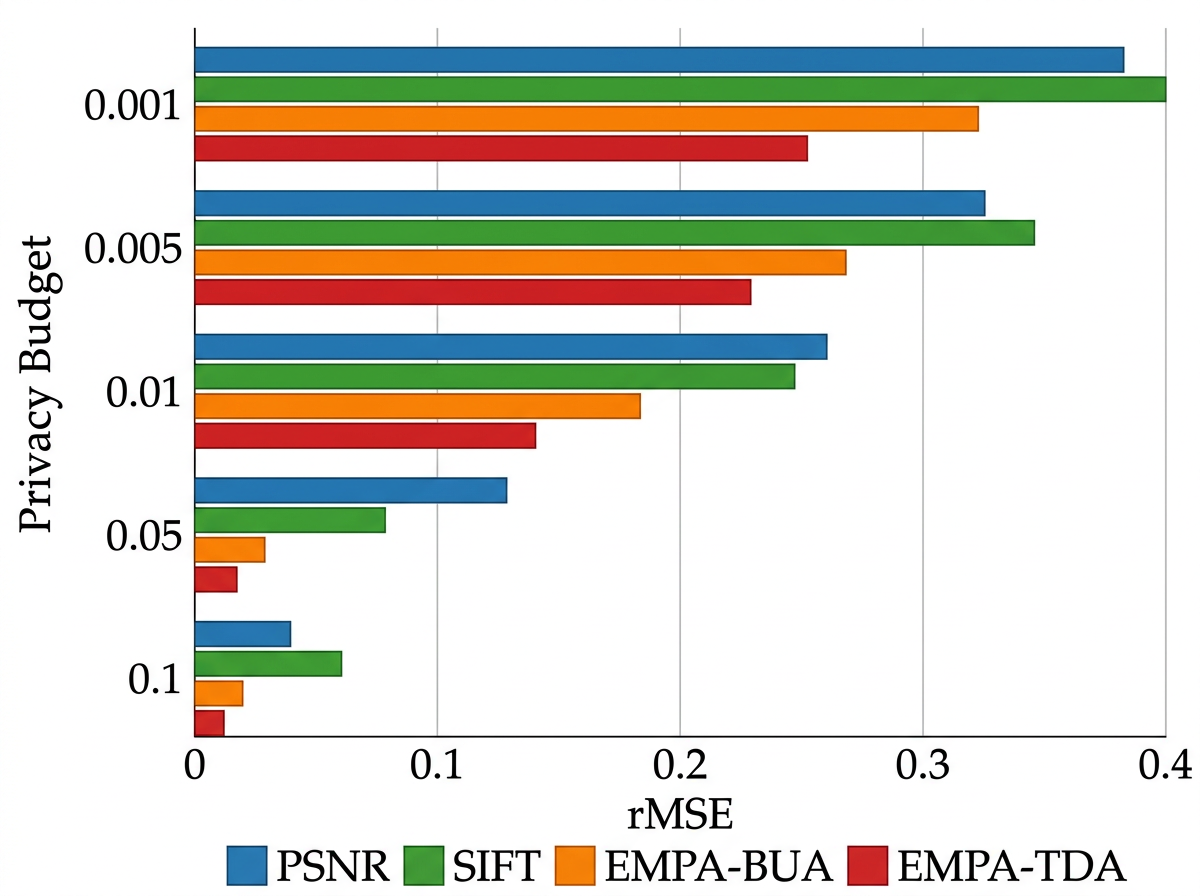
\includegraphics[width=0.8\columnwidth]{images/EMPA1.png}
\caption{Privacy budget vs.\ rMSE: TDA+EMPA and BUA+EMPA (COCO).}
\label{fig:empa1}
\end{figure}

\subsection{Results from Reproducible Script (Synthetic Hierarchical Features)}
\label{sec:scriptresults}

To validate the protocol in Section~\ref{sec:expdesign}, we ran the provided Python scripts on synthetic hierarchical features (4 layers, 200 samples, 8-D per layer, 30\% sensitive ratio) with Gaussian noise scaled by $1/\epsilon$. Table~\ref{tab:script} reports Chi-square statistic, K-L divergence, MMD, rMSE, and EMPA bias (BUA and TDA) for $\epsilon \in \{0.1, 0.01, 0.001\}$. As $\epsilon$ decreases, the injected noise magnitude increases ($\propto 1/\epsilon$), so rMSE between original and noised features grows (from 5.55 at $\epsilon=0.1$ to 555.3 at $\epsilon=0.001$). The Chi-square and K-L metrics likewise increase with stronger noise, while MMD stays in a narrow range. EMPA bias remains stable across the three budgets and is identical for BUA and TDA in this setup, indicating that both grouping strategies yield the same sensitive/non-sensitive partition on the synthetic data; the bias value (about 0.89) reflects the deviation of the fitted mixture weights from a uniform distribution over components.

Figure~\ref{fig:script_empa} plots the EMPA bias (vertical axis) against the privacy budget $\epsilon$ (horizontal axis, log scale) for BUA+EMPA and TDA+EMPA. Both curves overlap because the two strategies produce the same groups on this synthetic hierarchy; the flat trend shows that the bias is determined mainly by the group structure rather than the noise scale in this experiment. Figure~\ref{fig:script_metrics} provides a two-panel matplotlib figure: the left panel shows rMSE vs.\ $\epsilon$ (log scale on both axes), illustrating the sharp rise in reconstruction error as $\epsilon$ decreases; the right panel shows Chi-square, K-L divergence, and MMD vs.\ $\epsilon$, so that readers can compare how each baseline metric responds to the privacy budget. These figures were generated automatically by the script \texttt{plot\_paper\_figures.py} from the CSV output of \texttt{run\_experiments.py}; the scripts are available in the repository.

\begin{table}[t]
\centering
\caption{Metrics from reproducible script (synthetic hierarchical features).}
\label{tab:script}
\begin{tabular}{c|ccccc|cc}
\hline
$\epsilon$ & Chi-square ($\times 10^6$) & K-L & MMD & rMSE & (max gap) & EMPA (BUA) & EMPA (TDA) \\
\hline
0.1  & 12.9 & 1.78 & 0.0138 & 5.55 & -- & 0.894 & 0.894 \\
0.01 & 69.1 & 4.82 & 0.0212 & 55.5 & -- & 0.894 & 0.894 \\
0.001& 69.0 & 4.84 & 0.0217 & 555.3 & -- & 0.894 & 0.894 \\
\hline
\end{tabular}
\end{table}

\begin{figure}[t]
\centering
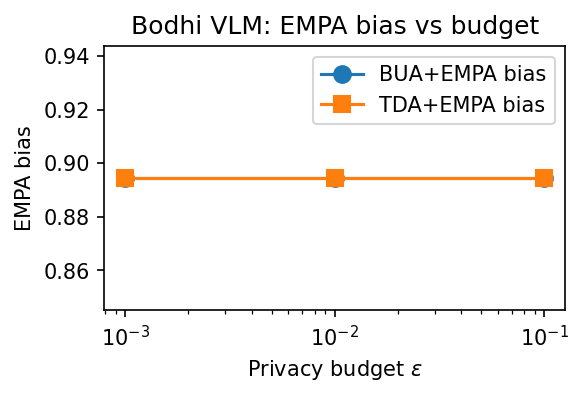
\includegraphics[width=0.85\columnwidth]{images/bodhi_vlm_empa_bias.png}
\caption{EMPA bias vs.\ privacy budget $\epsilon$ (log scale) from the reproducible script. The vertical axis is the bias output by EMPA (deviation of mixture weights from uniform); the horizontal axis is $\epsilon$. BUA+EMPA and TDA+EMPA coincide because the synthetic grouping yields the same partition.}
\label{fig:script_empa}
\end{figure}

\begin{figure}[t]
\centering
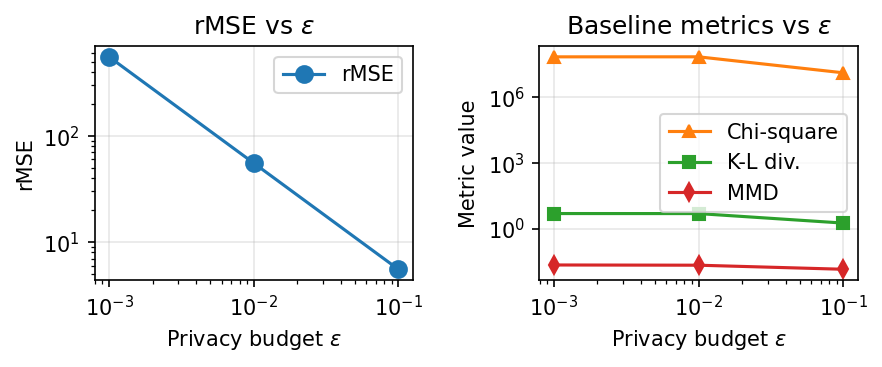
\includegraphics[width=0.98\columnwidth]{images/bodhi_vlm_metrics_vs_epsilon.png}
\caption{Left: rMSE between original and noised features vs.\ $\epsilon$ (log scale). Right: Chi-square statistic, K-L divergence, and MMD vs.\ $\epsilon$. Generated by \texttt{plot\_paper\_figures.py} from \texttt{bodhi\_vlm\_metrics.csv}.}
\label{fig:script_metrics}
\end{figure}

\subsection{Ablation and Membership Inference}
Ablation (removing TDA, BUA, or EMPA) shows that the full pipeline is needed for accurate budget assessment; removing EMPA increases deviation from the ground-truth budget (see ablation figure in supplementary). Membership inference attack (MIA) accuracy on TSDCRF vs.\ PPEDCRF is reported in the thesis; both sit above random (0.5), suggesting further work for stronger guarantees.

\section{Conclusion}
\label{sec:conclusion}

We presented Bodhi VLM, a privacy budget assessment framework that combines bottom-up (BUA) and top-down (TDA) feature search with an Expectation-Maximization Privacy Assessment (EMPA) method. The same pipeline applies to object detectors (FPN backbones) and to the vision tower of vision-language models (e.g., CLIP, LLaVA, BLIP). BUA and TDA produce sensitive/non-sensitive feature groups per layer; EMPA reconstructs the privacy-feature distribution and outputs a bias relative to the budget. On MOT20 and COCO, BUA and TDA show comparable behavior, with BUA slightly more sensitive; EMPA yields lower rMSE than Chi-square, K-L, and MMD. We provided an experimental protocol and Python scripts for reproducibility. Future work includes applying Bodhi VLM to full VLM training pipelines, one-run auditing, comparison with theoretical leakage lower bounds, and automated feedback to the preprocessing layer for adaptive $\epsilon$ tuning.

\bibliographystyle{IEEEtran}
\bibliography{ref}

\end{document}
